\section{Indledning}
C er et genial sprog\cite{C-bog}. Jeg ved at Nikolai elsker det! Måske det kan beregnes hvor meget?

\subsection{Hvor meget elsker Nikolai C?}
Lad os kigge på tallene. Hvis vi tager kvadratroden af produktet af $x$ og $69.420$ og sætter i anden, så får vi faktsik en funktion af, hvor meget Nikolai elsker C.

\begin{gather}
    \label{eq:nikolai}
    f(x) = (\sqrt{x \cdot 69.420})^2
\end{gather}

Vi kan se på formel \ref{eq:nikolai} at det altså er ret meget, som Nikolai elsker C. Lad os vise dette på en graf:

\begin{figure}[h!]
    \centering
    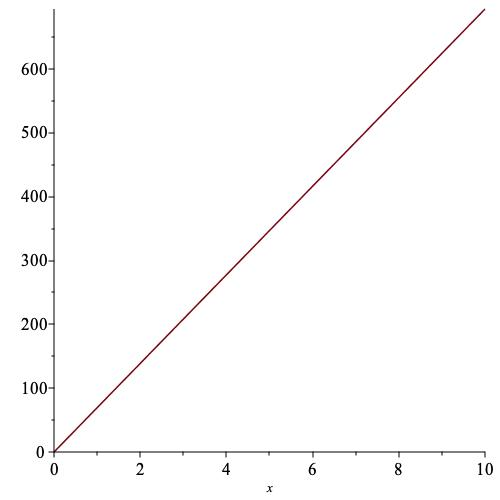
\includegraphics[width=0.8\linewidth]{Figurer/Nikolai-c.jpg}
    \caption{Graf der viser udviklingen af Nikolais kærlighed til C}
    \label{fig:nikolai-c}
\end{figure}

\noindent % Normalt er nye afsnit indrykket
Hvis vi ser på figur \ref{fig:nikolai-c} kan vi altså se, at det kun går fremad

\subsection{Programmering i C}
Lad os her vise et eksempel på noget C kode, så vi bedre kan forstå, hvorfor Nikolai elsker C så meget.

\begin{minted}{C}
#include <stdio.h>

int main(void) {
    printf("Hello, World!")
    
    return 0;
}
\end{minted}
\noindent
Det er især \mintinline{c}{int main(void)}, Nikolai elsker